
	% sampling
\section{Sampling}

\begin{frame}
	\frametitle{Sampling}
	\begin{itemize}
		\item \textbf{continuous signal} (normalized magnitude, length $L$ in seconds)
			\begin{align*}
				x(t)\in[-1,1],\quad t\in[0,L]
			\end{align*}
		\item \textbf{sampling rate} $f_{\textrm S}$, quantization of time (Audio CD: $44.1\kilo\hertz$)
			\begin{align*}
				t\rightarrow t_i=\frac{i-1}{f_{\textrm S}},\quad i\in\{1,\ldots,N\},\quad N=\lfloor Lf_{\textrm S}+1\rfloor
			\end{align*}
		\item \textbf{bits per sample} $n_{\textrm S}$, quantization of amplitude (Audio CD: $16\bit$)
			\begin{align*}
				x(t)\rightarrow x_i=\left\lfloor2^{n_{\textrm S}-1}x(t_i)\right\rceil
			\end{align*}
	\end{itemize}
\end{frame}

\begin{frame}
	\frametitle{Sampling}
	\begin{itemize}
		\item \textbf{example} (\texttt{dsp/matlab/sampling.m})
			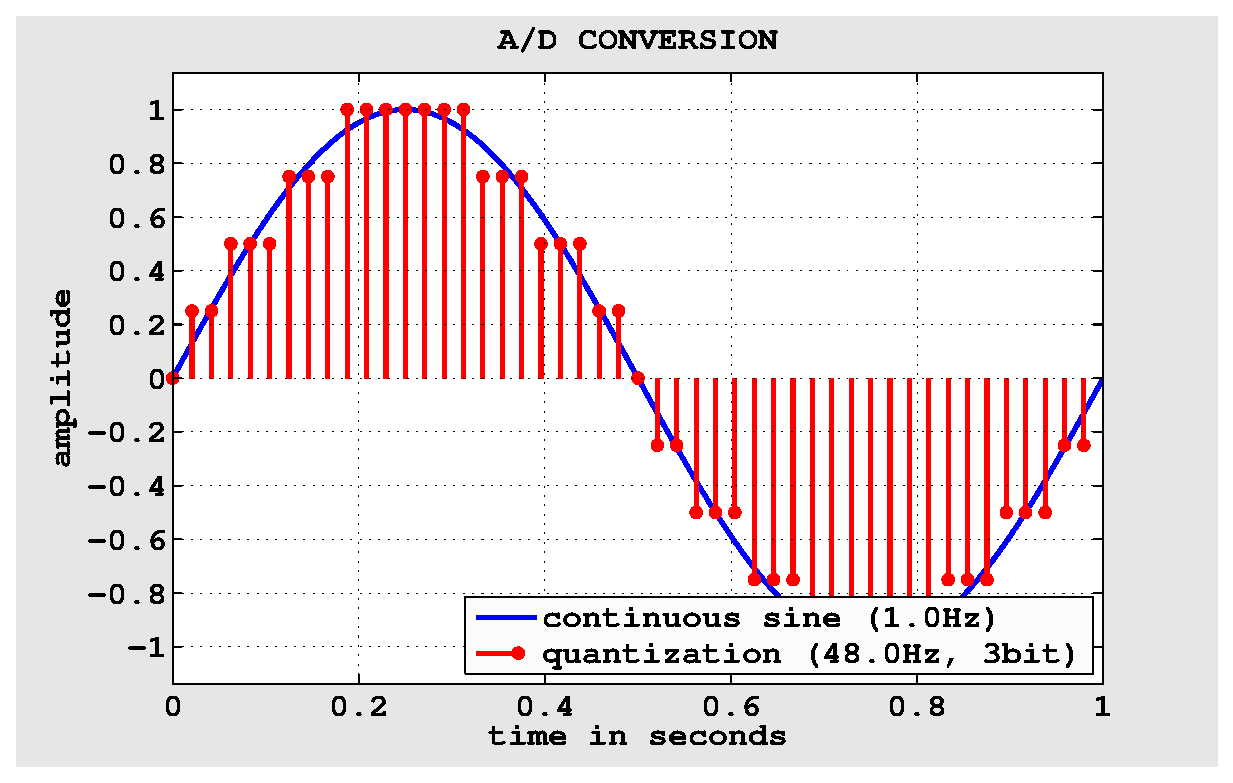
\includegraphics[width=4cm]{\imagedir/dsp/sampling_ad.eps}
			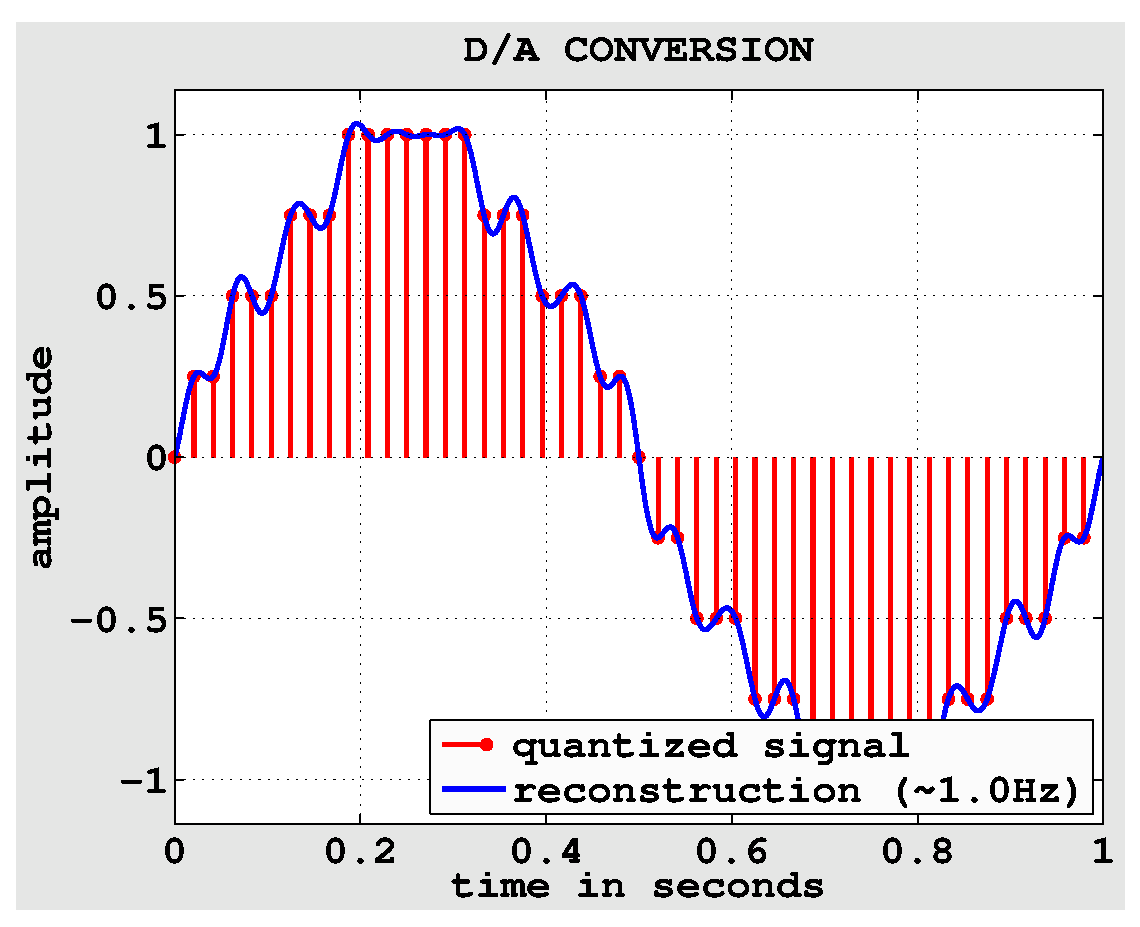
\includegraphics[width=4cm]{\imagedir/dsp/sampling_da.eps}
		\item \textbf{exercise}
			\begin{itemize}
				\item sampling theorem
				\item Nyquist frequency, aliasing
			\end{itemize}
	\end{itemize}
\end{frame}

